\documentclass{standalone}

\usepackage{tikz}

\begin{document}
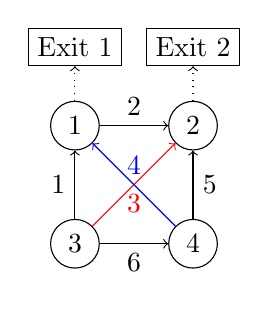
\begin{tikzpicture}

\node[draw, rectangle] (exit-1) at (0,2.5) {Exit 1};
\node[draw, rectangle] (exit-2) at (1.5,2.5) {Exit 2};

\node[draw, circle] (1) at (0,1.5) {$1$};
\node[draw, circle] (2) at (1.5,1.5) {$2$};
\node[draw, circle] (3) at (0,0) {$3$};
\node[draw, circle] (4) at (1.5,0) {$4$};

\draw[->] (3) to node[left] {$1$} (1);
\draw[->] (1) to node[above] {$2$} (2);
\draw[->,red] (3) to node[below] {$3$} (2);
\draw[->,blue] (4) to node[above] {$4$} (1);
\draw[->] (4) to node[right] {$5$} (2);
\draw[->] (3) to node[below] {$6$} (4);

\draw[->, dotted] (1) to (exit-1);
\draw[->, dotted] (2) to (exit-2);

\end{tikzpicture}
\end{document}
